%!TEX root = main.tex
%
% ### Research Method
% Where are we getting requirements from?  
% What will guide our design?  
% How will we evaluate the tool?  
%
\section{Research Method}

% Lage et diagram som http://daim.idi.ntnu.no/masteroppgave?id=6231 og Timeline masteroppgaven gjør. Altså hvordan vi har gått frem underveis. Skriv så litt om hver periode, hva vi har gjort etc. Veldig likt timeline bare ikke så mye. Dropp såå alle de subsectionsa under. Går sikkert an å bake inn litt fra de ulike stedene, de bør jo nevnes. F.eks research rigor etc. 

\subsubsection{Design as an artifact}
By definition, the result of design-science research in Information Science is:
\begin{quote}
A purposeful IT artifact created to address an important organizational problem. It must be described effectively, enabling its implementation and application in an appropriate domain.
\end{quote}
\cite{markusetal} identified that a developed artifact is only significant if there is questions like: Can it be constructed, can it perform appropriately and is the result important to the information science community. 
We will create a proof of concept prototype tool for promoting experienced-based learning from reflection based on project artifacts collected from version-control systems. Our goal was to create a tool that can discover new capabilites in the domain of reflection and experience-based learning, as well as support the existing capabilities in an efficient way. Evaluating the tool in \emph{real use} situations is necessary in order to discover if the artifact can enhance the reflection process as it is today. \\

\subsubsection{Research Guidelines}
The \emph{Design-Science Research Guidelines} presented in \cite{Esearch2004} will serve as the basis of this design-science research. The guidelines were created in order to assist researchers to understand the necessary requirements for effective design-science research. 

\subsection{Design as a research process}
Implementation of the application was done in development cycles, inspired be the regulative cycle presented by \cite{wieringa}, and is shown in \ref{regulativecycle}. 
The early parts of the development process was used to develop ideas and basic mock-ups of the application and its design. The initial prototype design was based heavily on the first concept and mockups created, in addition to recurring feedback from users and supervisors. Early parts of development resulted in a prototype with functionality for individual reflection use. The next goal was to incorporate teams and support collaborative reflection in the team, building and improving on the basic functionality present in the tool. In the later parts of the development, the focus was the integration of individual reflection notes, into the team collaborative data. This resulted in a tool for both individual and collaborative aspects for reflection and learning. We used the tool ourselves during development, as it would be used in a real world environment. In this way we ensure that all functionality is as expected, and also identify limitations in the design. 

Finally we performed a case study evaluation with computer-science students, and an expert review. Evaluating these separately provide us two sets of feedback which we can compare in order to possibly see if any patterns emerge. 
\begin{figure}[!htpb]
\label{regulativecycle}
\centering
	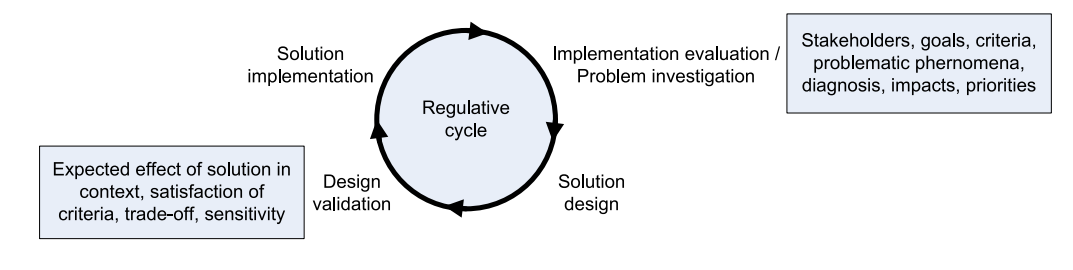
\includegraphics[width=\textwidth]{regulativecycle}
\caption{Regulativecycle development in Design-Science research}
\end{figure}

\subsection{Development process}
\begin{figure}[!htpb]
\label{researchmodel}
\centering
	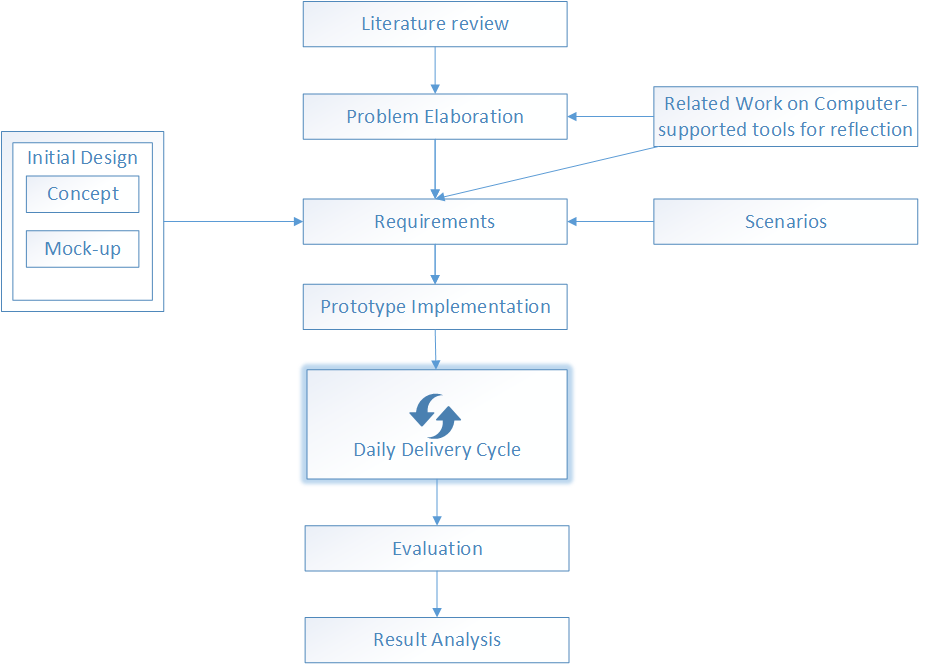
\includegraphics[width=\textwidth]{researchmodel_and_iterationcycle}
\caption{The researchmodel}
\end{figure}

\ref{researchmodel} shows the research model used for the development of our prototype from initial concept and ideas, to the final implementation and evaluation. The model depicts how we started the process by reading theory in order to get a better understanding the core concepts of reflection on experiences, and the learning from experiences(See \ref{chap:background} for the thesis background). We conducted a literature review (\ref{sec:literaturereview}) and looked at related work done on computer-supported tools for reflection and learning (\ref{sec:relatedwork}). On the basis of theory and previous work done, a problem elaboration was created (\ref{chap:problemelaboration}). The problem elaboration led us in turn to the process of creating the requirements for the application (\ref{chap:requirements}). The initial design with concept and mock-ups also helped identify requirements for the application, together with feedback from our supervisor. All implementations were then done conducted using a daily delivery cycle (\ref{sec:dailydeliverycycle}).

\subsection{Daily Delivery Cycle}
\label{sec:dailydeliverycycle}

\ref{iterationprocess} shows how our daily delivery cycle looked like. The cycle was inspired by the regulative cycle presented by Wieringa\cite{wieringa}. 
\begin{figure}[!htpb]
\label{iterationprocess}
\centering
	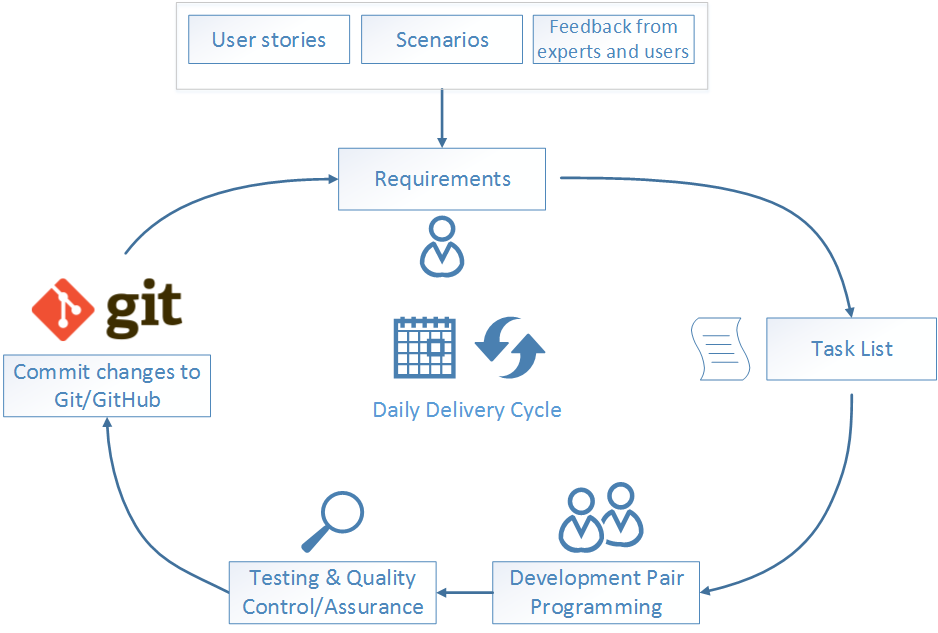
\includegraphics[width=\textwidth]{iterationprocess}
\caption{The daily delivery cycle}
\end{figure}

% Write some more about the daily cycle

\subsection{Evaluation}
% Read and rewrite this part if needed. Should be checked so that it fits with the rest of the chapter. 
Table 2 in \cite{Esearch2004} will be used as guidelines for evaluation of our prototype. 
During evaluation we will be using parts of the evaluation toolbox published by MIRROR\footnote{\url{http://www.mirror-project.eu/showroom-a-publications/downloads/finish/5/67}}. This toolbox is a specification of evaluation methodology and research tooling. 

\subsubsection{Observational}
Before and after the user evaluation of the tool, all test-subjects will be given a form with a set of questions to evaluate the application. We will be using core demographic questions, app usage, the most relevant app-specific questions, and also the reflection scale [\ref{reflectionscale}] from the toolbox. The reflection scale assesses participants' general tendency to reflect and the importance they place on reflection. Using this scale, allows us to see whether using the tool prime people to reflect more. Meaning: Does the tool increase the users tendency to reflect on experiences, both individually and as a team. Measuring this before and after using the tool implementation, allows us to measure the expected increase. \\*
Finally we will include the learning outcomes questions and the work behaviour questions, after the evaluation period.  

\subsubsection{Analytical}
We will perform a dynamic analysis on the data collected from server and user feedback. During use the application will provide simple usage-patterns on how the users use the application.
This will also help us in the analysis of the applications performance as well as its usefulness in the reflection and learning domains

\subsubsection{Testing}
During development we will continuously test the tool  to ensure that the user experience is as expected, as a means of quality assurance.
White Box testing will be executed during development of the application with artificial data to ensure that the function is working properly and as specified. 

\subsubsection{Descriptive}
Evaluation proposal with the students in IT2901 - A project course taken by computer science students on the Norwegian University of Science and Technology (NTNU). 
Students that accept to evaluate our tool, will use it for two weeks, with daily individual use and as a team after the two week period. This will allow us to measure the usage of our scenarios. 

Requirements: 
The first scenario does not require anything but a github repository and is doable both for single and for multiples in teams.
For scenario 2 we will require a team of at least 3 people in order to collect enough data. 
We have continuously been using and evaluating the tool ourselves, also a fellow student has been using it for a couple of weeks, so we have some additional evaluation
data also.
% Should be written more structured


% This should come last in the chapter, unsure of how much we need to have here. Incorporate as much as possible into parts above. 
\subsection{Problem relevance}
We want to explore how the collection and scaffolding of experiences connected to project artifacts can support collaborative reflection sessions. In order to revisit and learn from previous experiences we want to collect and scaffold experiences from users daily. Experiences and memories change over time, so collecting these experiences as quickly as possible is important. The tool will keep a copy of these experiences in order for users to revisit them at a later date, be it individually or in collaborative reflection sessions. These notes will be collected based on tags that are related to the experience being reviewed \cite{Hassan-montero2006}

\subsection{Research Contributions}
The main goal is to create a proof of concept application that will help users reflect on their past experiences individually and in collaborative reflection sessions by collecting experiences daily and revisiting them at any time. We will analyse the users experience and the evaluation results  in order to draw a conclusion on if multiple representations might help the users to reflect on their past experiences in a collaborative session.

\subsection{Research Rigor}
We will test the tool with a group of experts in the fields relevant and gather data during testing with this group and use this to evaluate the usefulness of the tool. This will serve as a good basis for analysis, triangulate and evaluate to look for relevant research results elsewhere.

\subsection{Research communication}
The proof of concept application will be available for testing along with a user guide, the whole process will be well documented and our research results will be made available.
Any limitations identified  will be documented along with the research results. 



